\documentclass{article}

\usepackage{listings}
\usepackage[english]{babel}
\usepackage{color}
\usepackage{graphicx}
\graphicspath{{img/}}

\interlinepenalty 10000

\definecolor{dkgreen}{rgb}{0,0.6,0}
\definecolor{gray}{rgb}{0.5,0.5,0.5}
\definecolor{mauve}{rgb}{0.58,0,0.82}

\lstset{frame=tb,
  language=Java,
  aboveskip=3mm,
  belowskip=3mm,
  showstringspaces=false,
  columns=flexible,
  basicstyle={\small\ttfamily},
  numbers=none,
  numberstyle=\tiny\color{gray},
  keywordstyle=\color{blue},
  commentstyle=\color{dkgreen},
  stringstyle=\color{mauve},
  breaklines=true,
  breakatwhitespace=true,
  tabsize=3
}

\title{Spyke (Babel Project) - Technical Documentation}
\author{La Pintade}
\date{5 October 2015 - 8 November 2015}

\begin{document}

  \maketitle
  \tableofcontents


  \newpage
  \section{About}
    This document is a technical documentation about Spyke.
    Spyke is a software developped by the La Pintade team, based in Nice.
    The team developped a Skype-like product in a month for the Epitech's Babel project.
 \bigskip

  We will firstly explain the project conception: it is divided in 2 parts. There is the Server and the Client. The server receives data from a client and transfers it to the others. Clients sends request to the server and get datas in order to call other clients.
  \newpage

  \section{Client}

  In this section, we will see in details what we used for the client and how it was thought.

  \subsection{Libraries chosen}

  \bigskip
  Port Audio
  \bigskip

  Firstly, we used Port Audio for sound related things. We chose it because it is an Open-Source Cross-Platform Audio library recognized and used by many such as the free audio editor Audacity. It helps us to get sound from the computer's microphone and to play it through it's speakers.

  \bigskip
  Since it is a C library, we had to encapsulate it so here it is: our encapsulation of Port Audio.
  \bigskip

  \begin{lstlisting}
    typedef float SAMPLE;
    namespace SoundDevice {
      const unsigned int channels = 2; //definition of Port Audio number of channels ( = 2 for stereo)
      const double sampleRate = 44100; //setting of Port Audio Rate to be compatible with Opus
    }

    class   ISoundDevice
    {
    public:
      virtual ~ISoundDevice() {};
      virtual void start() = 0;
      virtual void stop() = 0;
    };
  \end{lstlisting}

  \bigskip

  It has two simple methods start() and stop() in order to start and stop recording or start and stop playing sound.

  \newpage

  \bigskip
  Opus
  \bigskip

  Then we used Opus for the compression codec. We chose it because it is a totally open and highly versatile audio codec (Skype uses it). It helps us to encode and decode our sound recorded with Port Audio in order to send the packages encoded and to decode them once received.

  \bigskip
  Since it is also a C library, we had to encapsulate it too. This is our encapsulation of Opus:
  \bigskip

  \begin{lstlisting}
    namespace Encoder {
    }
    class   IEncoder
    {
      public:
      virtual ~IEncoder(){};
      virtual SEncoded encode(SDecoded) = 0;
      virtual SDecoded decode(SEncoded) = 0;
    };
  \end{lstlisting}

  \bigskip

  It has two methods encode() and decode() returning structures with encoded and decoded data.

  \newpage

  \bigskip
  Qt
  \bigskip

  Finally, we used Qt for the Graphical User Interface and QtNetwork for all the network related things. We chose it because it is basically ranked 1 of all cross-platform tools and known powerfull for UIs and applications that runs on any operating system. Moreover, it is a native C++ library so we don't have to encapsulate it. It helps us to build our GUI through a lot of Qt classes and to create TCP and UDP connections to server and clients.

  \bigskip
  Since it is a C++ library, we don't need to encapsulate it. However, here is the very beginning of our network TCP class. It shows an example on how we use Qt (obviously for network here).
  \bigskip

  \begin{lstlisting}
    class QTcpSocket;
    class NetworkServerHandler : public QObject, public INetwork // QObject
    {
      Q_OBJECT
      private:
      QObject *parent;
      QTcpSocket *_socket; // QTcpSocket
      std::string _host;
      unsigned int _port;
      bool          _connected;
      ...
  \end{lstlisting}

  \bigskip

  Our class NetworkServerHandler inherits from the QObject Qt class (and our Network abstraction INetwork) and we use a pointer to a QTcpSocket to create our socket.

  \newpage

  \subsection{Design choices}

  In this section, we will see how does the program looks like and why.
  Since it is a skype-like project, we decided to pursue in the idea of copying skype, even in the GUI design.

  \bigskip
  Here is the Login Screen
  \bigskip

  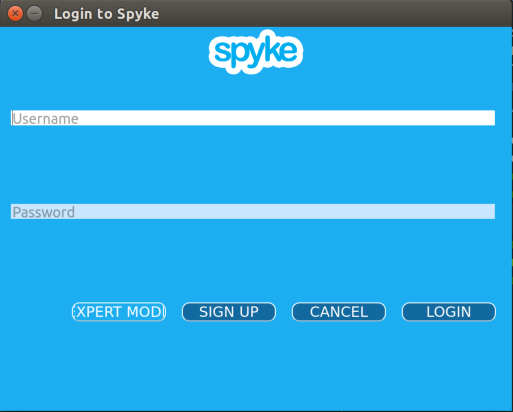
\includegraphics[width=350]{loginScreen}

  \bigskip
  As you can see, we used the same blue color as Skype.
  Buttons are the same as Skype except the Expert mode button, it's another feature that we added so that you can chose your server ip.
  \newpage

  The login, Sign in and expert mode views are really similar so we won't show all of them. If you want a detailed manual of how it looks, see the User's guide.

  \bigskip
  This is the screen once you are logged
  \bigskip

  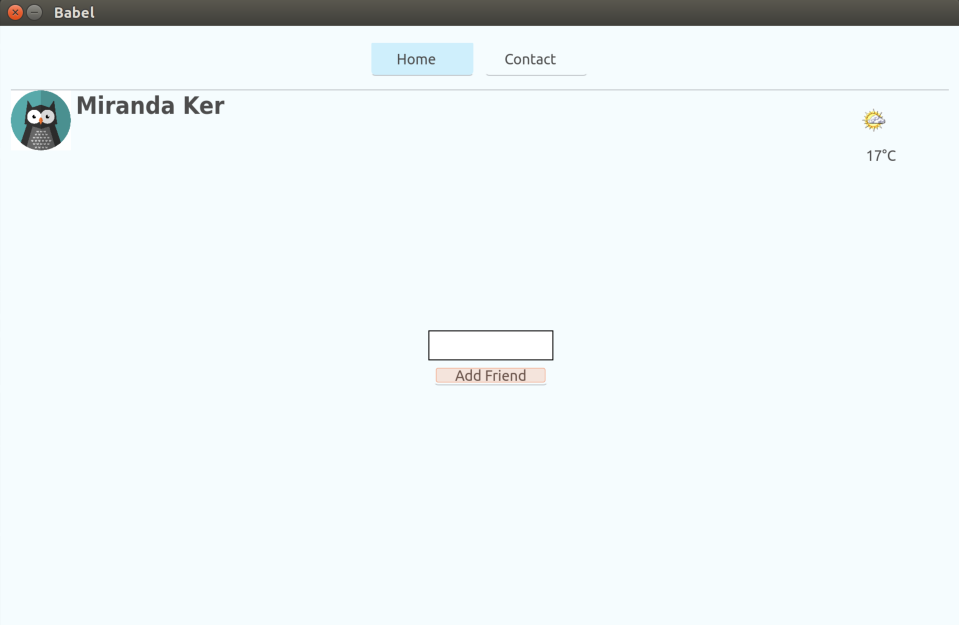
\includegraphics[width=350]{loggedScreen}

  \bigskip
  We chose the clearest (in our opinion) way to display informations: we cleaned as much as we could and we got this result; Your profile picture with your name, the field to add a friend, the meteo and the 2 pannel buttons which are Home and Contact.
  This allows the users to access every features like calling people or checking meteo the simplest way possible. For more informations check the User's guide.

  \newpage

  \subsection{Conception}

  \subsubsection{Architectural Patterns}

  In order to develop a professionnal project we used some architectural patterns.

  \bigskip
  We firstly used the Model-View-Controller(MVC) architectural pattern for implementing the user interface for the client.

 In our case, the model is the nested class User: it directly manages the data, logic and rules of the application independently of the user interface.
 Next comes the view, which here is all our GUI classes. They output a representation of the informations.
 The controller is the PTUser class: it accepts input and converts it to commands for the model or view.
 \bigskip

 Secondly, we used the Observer pattern with Qt. The GUI classes sends signals for every event that is happening to the slots from the PTUser class.

 \bigskip

 If you're new to the Observer pattern, here is a few reminders you should know:
 A signal is an observable event, or at least notification that the event happened.
 A slot is a potential observer, typically in the form a function to be called.
 You connect a signal to a slot to establish the observable- observer relationship.

 \newpage
 \subsubsection{TCP Connection}

 In this subsection, we will explain the TCP Connection part of the client. It is the directly related to the Server-Client communication part.

 At this point, you should know that the GUI classes handle events with the PTUser class using the Observer pattern.
 \bigskip

 Once those events received, the PTUser class uses the NetworkServerHandler class in order to send requests to the server.

 This NetworkServerHandler sends and receives the data to / from the server.

 However, the NetworkServerHandler class needs help to build proper strings that match the protocol so that the server understands what he receives.

 That's where we have the TCPProtocolHelper class: it builds the requests for the NetworkServerHandler.

 Note that in this part we don't need threads since Qt is already multithreaded.
 \bigskip

 The PTUser class has a NetworkServerHandler server attribute.
 The method int run(int ac, char **av) launches the program loop: ac and av are the arguments from the main, needed when initiating the Qt app.

 \bigskip
 The NetworkServerHandler class has a QTcpSocket *socket attribute and a TCPProtocolHelper request.
 The method int start(const std::string &host, unsigned int port) initiate the TCP connection with the server: host is the server ip and port is the port.
 The method void write(const std::string &request) sends the data to the server (writing on the socket): request is the string built by TCPProtocolHelper.
 The method void readyRead() reads data and calls the handleRequest() method from the TCPProtocolHelper class.
 \bigskip

 The TCPProtocolHelper class creates request with the createRequest() method and translate data with handleRequest().
 QByteArray createRequest(ProtocolType type) creates the request: type is an enum defining the type of the request.
 void handleRequest(qint8 type) treats the request from the server by calling the right function corresponding to the type using an array of function pointers.

 \newpage

 \subsubsection{UDP Connection}

 In this subsection, we will explain the UDP Connection part of the client. It corresponds to the client to client connection.
 It is in this part that we use PortAudio and Opus libraries.

 \bigskip
 Once the PTUser wants to establish a call, he uses the CallManager class.

 This CallManager class basically manage calls with different classes:

 \bigskip
 The NetworkClientHandler sends and receives the datas to / from the other client.
 Those datas are built by PTSoundInput; this class uses PortAudio to get the sound coming in the microphone and the classes Mutex and MutexLocker so they don't interrupt the app loop.
 However, the NetworkClientHandler class needs help to encode and decode data before sending it / transfering it.
 That's where we have the PTEncoder class: it encodes and decodes the audio datas.
 Finally, when the datas are ready the CallManager uses the PTSoundOutput to play the sound through speakers.
 \bigskip

 The CallManager class has many attributes to manage calls:

  \begin{lstlisting}
    NetworkClientHandler _client;
    PTSoundInput _input;
    PTSoundOutput _output;
    PTEncoder _encoder;
  \end{lstlisting}

  \bigskip
  The NetworkClientHandler is similar to the NetworkServerHandler seen above. However, it has a QUdpSocket *socket rather than a QTcpSocket since we want to establish an UDP connection between clients.
  Then it has the methods void write(const std::string &request) and void readyRead() doing the same as NetworkServerHandler methods (except it is for the client, obviously...)
  \bigskip

  The PTSoundInput class has an attribute PaStream *stream from PortAudio.
  Two methods void start() and void stop() simply start and stop recording audio.

  \bigskip

  PTEncoder has an OpusEncoder *encode attribute.
  It works simply with SEncoded encode(SDecoded) and SDecoded decode(SEncoded) to encode datas before sending it and to decode datas after receiving it.

  \bigskip

  The PTSoundOutput works the same as PTSoundInput except that start() and stop() output the decoded audio through speakers.

  \newpage
  \section{Server}

  In this section, we will see in details what we used to develop the server and how it was thought.

  \subsection{Libraries choosen}

  \bigskip
  Boost C++
  \bigskip

  The main library that we used for our server is Boost since it is a crossplatform really powerfull library for network and parsing purpose. It helps us to build a strong server with asynchronous multi client connections.

  \bigskip
  Since it is a C++ library, we don't have to encapsulate it. As with Qt for the Client side, Boost allows us to manage the network very easily: here are a few types that we use:
  \bigskip

  \begin{lstlisting}
    boost::asio::tcp::socket; // for our tcp socket
    boost::asio::io_service; // to manage the asynchrous service
    boost::asio::ip::tcp::acceptor; // for accepting new socket connections
    boost::system::error_code; // to manage errors
    boost::posix_time::ptime; // to get the date
  \end{lstlisting}

  \bigskip
  This is just examples on how we use Boost. If you want more informations, see the Conception part of the Server below.

  \newpage

  \subsection{Conception}

  Here, you will see how does the server work.

  \bigskip

  The Server class is the starting point of our server: it has an std::vector of Account* \_allAccounts corresponding to every account and an INetwork* \_net to handle the network part.

  \bigskip
  The Account class is full of attributes with getters and setters like a login, a password, an id, a list of contacts etc...

  \bigskip
  The Network class (which inherits from INetwork) has a TCPServer *server attribute and a void start() method. This method launches the loop of the server.

  \bigskip
  The TCPServer class has a list of TCPConnection and a boost::asio::ip::tcp::acceptor for attribute, a void startAccept() and a void handleAccept(TCPConnection::pointer newConnection, const boost::system::errorcode &error) methods in order to accept new connections and push them into the list of TCPConnection.

  \bigskip
  Every TCPConnection has a boost tcp socket and a boost asio streambuf as attribute. The methods void asyncWrite(const std::string &message) and void asyncRead() are used to send and receive request.

  \bigskip
  Once the request received, we need to check if it is a valid one. That's why we have a VerifyRequest class which only have one method: void verify(const std::string &request) const. If the request is not valid (according to the protocol) it is not treated.

  \bigskip
  Now that we know the request received is valid, we need to identify it: the DataFromClient class (which is created in the verify() method from VerifyRequest) determines the clientID, the Type and the Data in the request.
  \begin{lstlisting}
    void DetermineType(const std::string &);
    void DetermineData(const std::string &);
    void DetermineClientID(const std::string &);
  \end{lstlisting}

  All of those methods take the request as a parameter and fill the class attribute that correspond.

  \bigskip
  Once the request identified, the DataFromClient constructor calls the method void methodChecker(DataFromClient &fromClient) from the ProtocolClient class.
  This method calls the right function depending on the fromClient.type. It has an array of function pointers corresponding to every request possible in the prototype.

  \bigskip
  Now that the request has been independently treated, we need to prepare a response. The Response class has a method setResponse() that sets the \_reponse attribute according to the protocol.

  \bigskip
  Finally, we need to send the response to the client ! That's why the Sender class (with a method void send(Response *response)) sends the response using the asyncWrite() method from TCPConnection.

  \newpage

  \subsection{A typicall request example}

  Now that you know how does the server work, we will show you a concrete simple example on the path of a request.

  \bigskip
  The 15th request: Modify Status

  \bigskip
  TCPConnection reads the request that just arrived.

  \bigskip
  VerifyRequest checks the header of the request.

  \bigskip
  Since VerifyRequest said it's ok, DataFromClient analyze the request and parse it.

  \bigskip
  Now ProtocolClient only has to call the modifyStatus function.

  \bigskip
  Response and Sender are in charge of sending success to the client.

  \bigskip
  The request Modify Status has now been treated, your status has changed.

\end{document}
